\documentclass{article}

\usepackage{tikz}
\usetikzlibrary{decorations.pathreplacing}

\definecolor{myLightGray}{RGB}{191,191,191}
\definecolor{myGray}{RGB}{160,160,160}
\definecolor{myDarkGray}{RGB}{144,144,144}
\definecolor{myDarkRed}{RGB}{167,114,115}
\definecolor{myRed}{RGB}{255,58,70}
\definecolor{myGreen}{RGB}{0,255,71}

\begin{document}

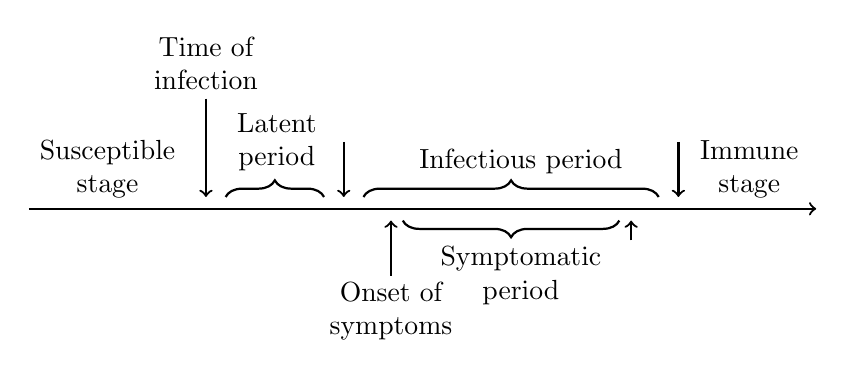
\begin{tikzpicture}[scale=1]
\node[align=center] at (1,0.5) {Susceptible\\stage};
\node[align=center] at (2.25,1.85) {Time of\\infection};
\draw [thick,->] (2.25,1.4) -- (2.25,0.15);
\node[align=center] at (3.15,0.85) {Latent\\period};
\draw [thick,decorate,decoration={brace,amplitude=6pt,raise=0pt}] (2.5,0.15) -- (3.75,0.15);
\draw [thick,->] (4,0.85) -- (4,0.15);
\node[align=center] at (6.25,0.6) {Infectious period};
\draw [thick,->] (8.25,0.85) -- (8.25,0.15);
\node[align=center] at (9.15,0.5) {Immune\\stage};
\draw [thick,decorate,decoration={brace,amplitude=6pt,raise=0pt}] (4.25,0.15) -- (8,0.15);
\draw [thick,->] (0,0) -- (10,0);
\draw [thick,->] (4.6,-0.85) -- (4.6,-0.15);
\draw [thick,->] (7.65,-0.4) -- (7.65,-0.15);
\draw [thick,decorate,decoration={brace,amplitude=6pt,raise=0pt,mirror}] (4.75,-0.15) -- (7.5,-0.15);
\node[align=center] at (6.25,-0.85) {Symptomatic\\period};
\node[align=center] at (4.6,-1.3) {Onset of\\symptoms};
\end{tikzpicture}

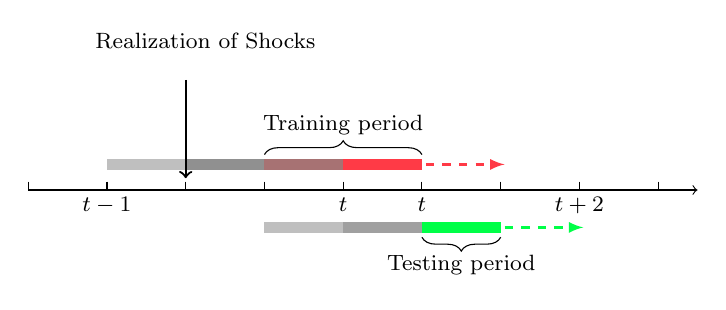
\begin{tikzpicture}[%
    every node/.style={
        font=\footnotesize,
        text height=1ex,
        text depth=.25ex,
    },
]
% draw horizontal line   
\draw[->] (0,0) -- (8.5,0);

% draw vertical lines
\foreach \x in {0,1,...,8}{
    \draw (\x cm,3pt) -- (\x cm,0pt);
}

% place axis labels
\node[anchor=north] at (1,0) {$t-1$};
\node[anchor=north] at (4,0) {$t$};
\node[anchor=north] at (5,0) {$t$};
\node[anchor=north] at (7,0) {$t+2$};

% draw scale above
\fill[myLightGray] (1,0.25) rectangle (2,0.4);
\fill[myDarkGray] (2,0.25) rectangle (3,0.4);
\fill[myDarkRed] (3,0.25) rectangle (4,0.4);
\fill[myRed] (4,0.25) rectangle (5,0.4);
\draw[myRed,dashed,thick,-latex] (5.05,0.325) -- (6.05,0.325);

% draw scale below
\fill[myLightGray] (3,-0.4) rectangle (4,-0.55);
\fill[myGray] (4,-0.4) rectangle (5,-0.55);
\fill[myGreen] (5,-0.4) rectangle (6,-0.55);
\draw[myGreen,dashed,thick,-latex] (6.05,-0.475) -- (7.05,-0.475);

% draw curly braces and add their labels
\draw[decorate,decoration={brace,amplitude=5pt}] (3,0.45) -- (5,0.45)
    node[anchor=south,midway,above=4pt] {Training period};
\draw[decorate,decoration={brace,amplitude=5pt}] (6,-0.6) -- (5,-0.6)
    node[anchor=north,midway,below=4pt] {Testing period};
    
% Add Lines
\node[align=center] at (2.25,1.85) {Realization of Shocks};
\draw [thick,->] (2,1.4) -- (2,0.15);

\end{tikzpicture}



Use this as template

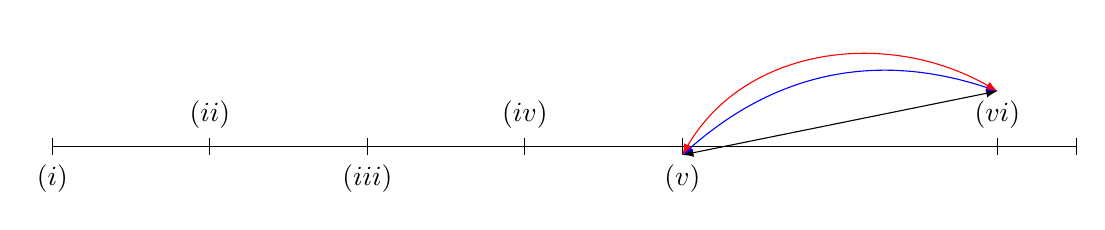
\begin{tikzpicture}
\draw (0,0) -- (13,0);
\foreach \x in {0,2,4,6,8,12,13}
  \draw (\x cm,3pt) -- (\x cm,-3pt);
\draw (0,0) node[below=3pt] (a) {$(i)$} node[above=3pt] {};
\draw (2,0) node[below=3pt] (b) {} node[above=3pt] {$(ii)$};
\draw (4,0)  node[below=3pt]  {$(iii)$} node[above=3pt] (c) {};
\draw (6,0) node[below=3pt](d) {} node[above=3pt] {$(iv)$};
\draw (8,0) node[below=3pt](e) {$(v)$} node[above=3pt] {};
\draw (12,0) node[above=3pt] (f) {$(vi)$} node[below=3pt] {};
\draw[latex-latex]
  (e.north) -- (f.north);
\draw[latex-latex,blue]
  (e.north) to[bend left] (f.north);
\draw[latex-latex,red]
  (e.north) to[out=60,in=150] (f.north);
\end{tikzpicture}\qquad

\linebreak



Use this as template

\begin{tikzpicture}
\draw (0,0) -- (13,0);
\foreach \x in {0,2,4,6,8,12,13}
  \draw (\x cm,3pt) -- (\x cm,-3pt);
\draw (0,0) node[below=3pt] (a) {$(i)$} node[above=3pt] {};
\draw (2,0) node[below=3pt] (b) {} node[above=3pt] {$(ii)$};
\draw (4,0)  node[below=3pt]  {$(iii)$} node[above=3pt] (c) {};
\draw (6,0) node[below=3pt](d) {} node[above=3pt] {$(iv)$};
\draw (8,0) node[below=3pt](e) {$(v)$} node[above=3pt] {};
\draw (12,0) node[above=3pt] (f) {$(vi)$} node[below=3pt] {};
\draw[latex-latex]
  (e.north|-f.north) -- (f.north);
\draw[latex-latex,blue]
  (e.north|-f.north) to[bend left] (f.north);
\draw[latex-latex,red]
  (e.north|-f.north) to[out=60,in=120] (f.north);
\end{tikzpicture}




Use this as template

\begin{tikzpicture}
\draw (0,0) -- (12,0);
\foreach \x in {0,3,6,9,12}
  \draw (\x cm,2pt) -- (\x cm,-2pt);

\node[align=center] at (1.5, 1) { Asset Choices \\ $k, b$ };

\node[align=center] at (3, 2.1) {$\epsilon$ \\ realized};
\draw [thin, -] (3, 1.6) -- (3, 0);

\node[align=center] at (4.5, 1) {Wealth \\ Realization \\ $\Lambda_t(k, b, \epsilon)$ };

\node[align=center] at (6, 1.8) {$r^I$ \\ realized};
\draw [thin, dashed] (6, 1.3) -- (6, 0);

\node[align=center] at (7.5, 1) {Asset \\ Choices \\ $k'(\Lambda, R^I, \epsilon)$ \\ $b'(\Lambda, R^I, \epsilon)$ };

\node[align=center] at (9, 2.1) {$\epsilon_{t+1}|\epsilon_{t}$ \\ realized};
\draw [thin, -] (9, 1.6) -- (9, 0);

\draw (0,0) node[below=3pt] (a) {$(i)$} node[above=3pt] {};
\draw (3,0) node[below=3pt] (b) {$(ii)$} node[above=3pt] {};
\draw (6,0)  node[below=3pt]  {$(iii)$} node[above=3pt] (c) {};
\draw (9,0) node[below=3pt](d) {$(iv)$} node[above=3pt] {};


\draw (12,0) node[below=3pt](e) {$(v)$} node[above=3pt] {};

\draw[latex-latex]
  (e.north|-f.north) -- (f.north);
\draw[latex-latex,blue]
  (e.north|-f.north) to[bend left] (f.north);
\draw[latex-latex,red]
  (e.north|-f.north) to[out=60,in=120] (f.north);
\end{tikzpicture}

\end{document}